%%%%%%%%%%%%%%%%%%%%%%%%%
% Dokumentinformationen %
%%%%%%%%%%%%%%%%%%%%%%%%%
\newcommand{\titleinfo}{OOAD - Zusammenfassung}
\newcommand{\authorinfo}{Schmidt J\"urg \& DIE Schweisser, Hannes, Gwerder, K\"orner, Niedermann}
\newcommand{\versioninfo}{$Rev: 1.0 $ | 
						gem\"ass Unterricht Martin Zimmermann/HS2012}  


%%%%%%%%%%%%%%%%%%%%%%%%%%%%%%%%%%%%%%%%%%%%%
% Standard projektübergreifender Header für
% - Makros 
% - Farben
% - Mathematische Operatoren
%
% DORT NUR ERGÄNZEN, NICHTS LÖSCHEN\newpage
%%%%%%%%%%%%%%%%%%%%%%%%%%%%%%%%%%%%%%%%%%%%%
\include{header/header}
\usepackage{enumitem}
\usepackage{wasysym}

\setlist{
	style=multiline,
	topsep=0pt,
	leftmargin=4.5cm,
	rightmargin=2cm
}

\usepackage{listings}
%\usepackage{textcomp}
\newcommand{\balzert}[1]{$_{\textcolor{red}{\mbox{\small{Balzert S. #1}}}}$}
\definecolor{lbcolor}{rgb}{0.92,0.92,0.92}
\lstset{
	backgroundcolor=\color{white},
	tabsize=4,
	rulecolor=,
	language=c++,
    basicstyle=\scriptsize,
    upquote=true,
    aboveskip={0.5\baselineskip},
    columns=fixed,
    showstringspaces=false,
    extendedchars=true,
    breaklines=true,
    prebreak = \raisebox{0ex}[0ex][0ex]{\ensuremath{\hookleftarrow}},
    frame=single,
    showtabs=false,
    showspaces=false,
    showstringspaces=false,
    identifierstyle=\bfseries\ttfamily,
    keywordstyle=\color[rgb]{0,0,1},
    commentstyle=\color[rgb]{0.133,0.545,0.133},
    stringstyle=\color[rgb]{0.627,0.126,0.941},
}

%\newcommand{\balzert}[1]{$_{\textcolor{red}{\mbox{\small{Balzert S.#1}}}}$}
\newcommand{\Balzert}[1]{${\textcolor{red}{\mbox{Balzert S.#1}}}$}

\begin{document}
\maketitle
\tableofcontents

\section{C++ CheatSheet}

\subsection{Header Files}
\begin{multicols}{2}
	\textbf{Include-Guard:}
	\begin{lstlisting}
	#ifndef MeinHeader_H
	#define MeinHeader_H
	// Ganzer Inhalt vom Header
	#endif
	\end{lstlisting}
	
	\textbf{Header und using namespace:} \\
	Kein \lstinline!using namespace std;! Wenn eine Funktion aus
	dem diesem Namespace gebraucht wird kann mit dem vollen Namen darauf
	zugegriffen werden. (\lstinline!std::cout << "..." << std::endl;!)
\end{multicols}


\subsection{Unterschied Statisch - Dynamisch}
\begin{multicols}{2}
\textbf{Statisch:}
\begin{lstlisting}
ClassA a;
a.foo(); // Funktionsaufruf
bar(&a); // Uebergabe von this
\end{lstlisting}

\textbf{Dynamisch:} 
\begin{lstlisting}
ClassA* a = new A();
a->foo(); // Funktionsaufruf
bar(a); // Uebergabe von this
\end{lstlisting}
\end{multicols}

\subsection{Assoziationen}
\subsubsection{"`0..1:0..1"'}
\begin{multicols}{2}
Vorwärtsdekleration wird gebraucht, wenn zwei Klassen sich gegenseitig referenzieren. \\

\textbf{Header A:}
\begin{lstlisting}
class B; // Vorwaertsdeklaration

class A{
	public:
	    A();
		void setB(B* pB);
		B* getB();
		
	private:
		B* mB; // Pointer auf B-Objekt
};
\end{lstlisting}

\textbf{Implementation:}
\begin{lstlisting}
void A::setB(B* pB) {
	mB = pB;
}
\end{lstlisting}

\columnbreak
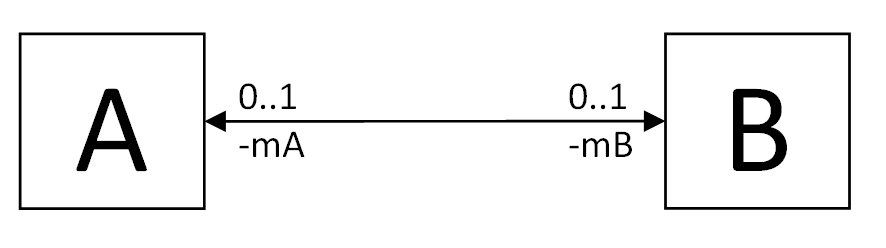
\includegraphics[width=5cm]{./bilder/Assozi_01_01.png}

\textbf{Header B:}
\begin{lstlisting}
class A; // Vorwaertsdeklaration

class B {	
	public:
		B();
		void setA(A* pA);
		A* getA();
		
	private: 
		A* mA; // Pointer auf A-Objekt
};
\end{lstlisting}

\textbf{Aufruf:}
\begin{lstlisting}
A a;
B b;
a.setB(&b);
\end{lstlisting}
\end{multicols}

\subsubsection{"`1:0..1"'}
Eine 1:0..1 Assoziation kann ähnlich wie eine 0..1:0..1 Assoziation
implementiert weden. Wobei auf der "`1 Seite"' die andere Klasse direkt im
Konstruktor mitgegeben wird. Ein Setter wird auf der B-Seite nicht mehr
gebraucht! Achtung: untenstehende Implementation zeigt nur schematisch auf wie
es funktioniert. Copy- und Zuweisungskonstruktor müssten auch noch korrekt
implementiert werden.
\begin{multicols}{2}
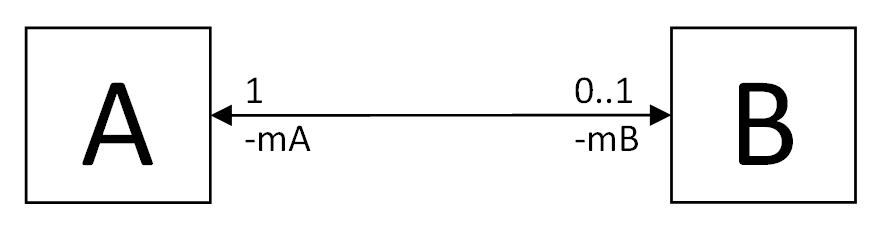
\includegraphics[width=5cm]{./bilder/Assozi_1_01.png}\\
\textbf{Header B (Muss Assoziation)}
\begin{lstlisting}
// ...
class B {
	public: 
		A* getA();
		B(A* pa);		// Konstruktor
	
	private:
		A* mA;		
		B();			// Default Konstruktor
}
\end{lstlisting}
\columnbreak
\textbf{Implementation B (Muss Assoziation)}
\begin{lstlisting}
B::B(A* pA)
: mA(pA)
{
	mA->setB(this); 
	// Kann auch im im Aufruf erfolgen
}
\end{lstlisting}

\textbf{Aufruf:}
\begin{lstlisting}
	A a;
	B b(&a);
\end{lstlisting}
\end{multicols}

\newpage

\subsubsection{"`0..1:0..n"'}
\begin{multicols}{2}
\textbf{Header A:}
\begin{lstlisting}
class B; // Vorwaertsdeklaration

class A{
	private:
		B* mB[n]; // Pointerarray auf B-Objekte
	
	public:
	    A();
		void addB(B* pB);
		void removeB(B* pB);
};
\end{lstlisting}

\textbf{Implementation:}
\begin{lstlisting}
A::A() {
	for(int i = 0; i<n; i++) {
		// Alle Werte auf 0 initialisieren
		mB[i] = 0; 
	}
}

// fuer removeB sinngemaess (->setA(0); mB[i]=0)
void A::addB(B* pB) {
	for(int i = 0; i<n; i++) {
		if(mB[i] == 0) {
			mB[i] = pB;
			mB[i]->setA(this);
			return;
		}
	}
}
\end{lstlisting}

\columnbreak
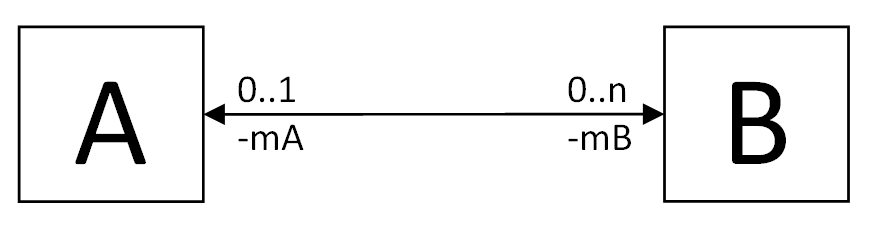
\includegraphics[width=5cm]{./bilder/Assozi_01_0n.png}\\
\textbf{Header B:}
\begin{lstlisting}
class A; // Vorwaertsdeklaration

class B {
	private: 
		A* mA; // Pointer auf A-Objekt
		
	public:
		B();
		void setA(A* pA);
		A* getA();
};
\end{lstlisting}

\textbf{Aufruf:}
\begin{lstlisting}
A a;
B b1;
B b2;
a.addB(&b1);
a.addB(&b2);
a.removeB(&b2);
// ...
\end{lstlisting}
\end{multicols}

\subsection{Vererbung}
\begin{multicols}{2}
\textbf{Basisklasse}
\begin{lstlisting}
	class: Fahrzeug
	{
	public:
			 Fahrzeug(int pGewicht);
		void setGewicht(int pGewicht);
	
	private:
		int mGewicht;
	};
\end{lstlisting}

\columnbreak

\textbf{abgeleitete Klasse}
\begin{lstlisting}
	class: Auto : public Fahrzeug
	{
	public:
			 Auto(int pPersonen, int pGewicht);	
		void setPersonen(int pPersonen);
		
	private:
		int	mPersonen;
	}	
\end{lstlisting}
\end{multicols}

\textbf{Aufruf}
\begin{lstlisting}
	Auto.setGewicht(42);
	Auto.setPersonen(4);
\end{lstlisting}





% Section OOA
% Objekt Orientierte Analyse

\section{OOA}

\subsection{Ziel der Analyse}
  \begin{itemize}[leftmargin = 0.5cm]
    \item Wünsche und Anforderungen an  ein neues System ermitteln und beschreiben
    \item Bei Modellbildung bewusst \textbf{alle} Aspekte der Implementierung ausklammern
    \item System als ideal anschauen. D.h keine Verzögerungen, keine Fehler, unendlicher Speicher
  \end{itemize}
  
\subsection{Zeil der OOA}
  Ziel ist es, das zu realisierende Problem zu verstehen und in einem OOA-Modell zu beschreiben.
  
\subsection{OOA Modelle}
  \begin{description}
    \item[statisches Modell] 
      beschreibt $\ldots$
      \begin{description}[leftmargin=0.5cm]
        \item[$\ldots$] die Klassen des Systems
        \item[$\ldots$] die Assoziation zwischen den Klassen
        \item[$\ldots$] die Generalisierung (Vererbung)
      \end{description}
      ausserdem enthält es die Daten des Systems (Attribute)
     
    \item[dynamisches Modell]
      \begin{itemize}[leftmargin=0.5cm]
        \item zeigt die Funktionsabläufe
        \item Use-Cases beschreiben die durchzuführenden Aufgaben
        \item Aktivität beschreibt die Ausführung von Funktionalität und Verhalten
        \item Szenario zeigen wie Objekte miteinander kommunizieren
        \item Zustandsautomaten beschreiben in der Analyse die Reaktion eines Objektes auf verschiedne Ereignisse
      \end{itemize}
      
    \item[OOA-Modell]
      \begin{itemize}[leftmargin=0.5cm]
        \item beschreibt die essenzielle Struktur und Semantik des Problems, aber noch keine technische Beschreibung
        \item enthält keinerlei Optimierung für das verwendete Computersystem oder die benutzte Basissoftware
        \item bildet fachliche Lösung des zu realisierenden Systems
      \end{itemize}
      
    \item[primitive Datentypen]
      \begin{itemize}[leftmargin=0.5cm]
        \item Boolean
        \item String
        \item Integer
        \item UnlimitedNatural
      \end{itemize}
  \end{description}
  
\subsection{Attribut \balzert{26}}
  \begin{description}
    \item[Attribut] 
      Beschreibt Daten die von den Objekten der Klasse angenommen
      werden können. Alle Objekte einer Klasse haben dieselben Attribute, können
      aber unterschiedliche Attributwerte haben.
    \item[Klassenattribut] 
      enn nur ein Attributwert für alle Objekte einer Klasse
      existiert. Sie existieren auch, wenn es zu einer Klasse noch keine Objekte gibt.
    \item[abgeleitets Attribut]
      kann zu jeder Zeit aus anderen Attributwerten berechnet werden. Wird mit \textbf{/zahl} geschrieben.  
    \item[Eigenschaftswerte von Attributen]
      siehe \Balzert{29}      
    \item[Multiplizität]
      [0..n] $\rightarrow$ spezifiziert, [0..*] $\rightarrow$ unspezifiziert
  \end{description}
  
\subsection{Klasse \balzert{23}}
  Eine Klasse ist eine Vorlage für ein Objekt.
  \begin{description}
    \item[Operation] 
      Eine Funktion die auf alle Attributwere eines Objekts Zugriff hat.
    \item[Klassenoperation] 
      Eine Operation, die der jeweiligen Klasse zugeordnet ist kann nicht auf 
      ein einzelnes Objekt der Klasse angewendet werden kann. 
    \item[Verhalten] 
      Das Verhalten der Klasse ist die Menge aller Operationen
    \item[Abstrakte] 
      Von einer abstrakten Klasse können keine Objekte erzeugt werden.
    \item[Basisklasse] 
      Vererbt abgeleiteten Klassen Attribute und Operationen
  \end{description}
  
\subsection{Objekt \balzert{20}}
	Ein Objekt wird aus einer Klasse erzeugt, ist also ein Exemplar einer Klasse.
	\begin{description}
		\item[Zustand] 
      Bestimmt durch seine Attributwerte und seine Objektbeziehungen zu anderen Objekten
		\item[Verhalten] 
      Die beobachtbaren Effekte aller Operationen bestimmt durch die Operationsaufruf, 
      auf die diese Klasse bzw. deren Objekte reagieren.
		\item[Objektidentität] 
      jedes Objekt hat eine Identität, welche einzigartig ist (unique)
	\end{description}
	
\subsection{Komponente}
  Ist ein Softwarebaustein, der über klar definierte Schnittstellen Verhalten (Funktionalität) bereitstellt.
  interface component
  
\subsection{Assoziation \balzert{42}}
	Modelliert Objektbeziehungen zwischen Objekten einer oder mehrerer Klassen.
	Jede Assoziation wird durch Mutliplizitäten, einen optionalen Namen oder Rollennamen
	beschrieben.
  \begin{description}
    \item[binäre Assoziation] 
      Assoziation zwischen 2 Objekten
    \item[ternäre Assoziation] 
      Assoziation zwischen 3 Objekten
    \item[n-äre Assoziation] 
      zwischen n Objekten
    \item[reflexive Assoziation] 
      Verbindet zwei Objekte der gleichen Klasse
    \item[Assoziationsklasse]
      \parbox{5cm}{Besitzt die Eigenschaften einer Assoziation und einer Klasse}
      \hspace{0.5cm}
      \parbox{9cm}{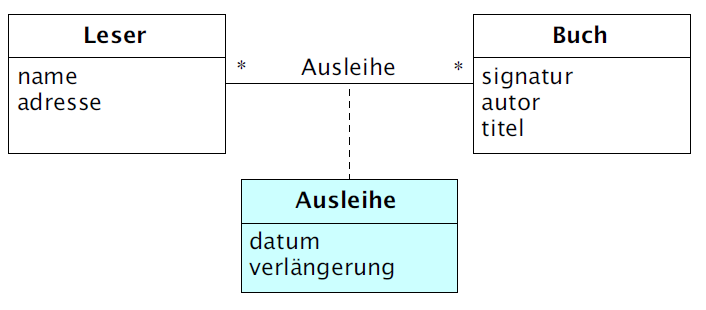
\includegraphics[width=6cm]{./bilder/Assoziationsklasse.png}}
    \parbox{6cm}{
      \item[Aggregation] 
        Sonderfall der Assoziation. "`ist Teilvon"' oder "`besteht aus"'.
      \item[Komposition] 
        starke Form der Aggregation. Beim löschen werden alle Teile gelöscht werden. 
        Jedes Teil kann nur zu einem Ganzen gehören}
    \parbox{9cm}{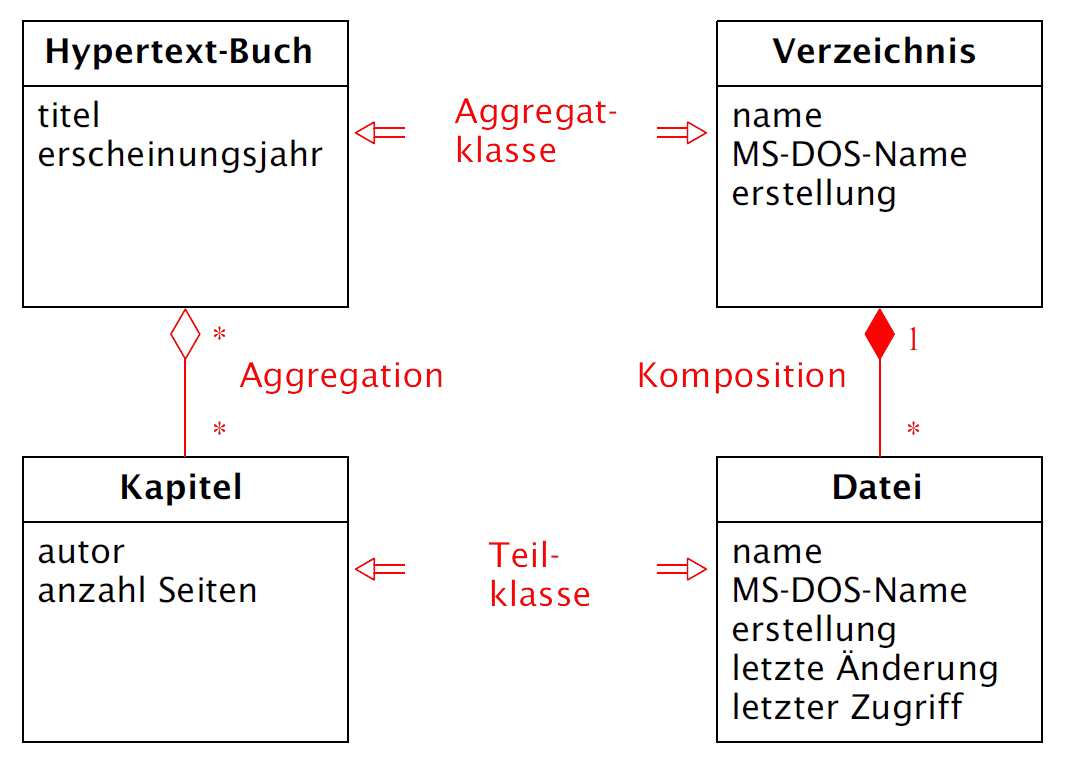
\includegraphics[width=6cm]{./bilder/Aggregation_Komposition.png}}
    \item[Navigationsrichtung] 
      Das erzeugen des einen erzwingt die Erzeugung des Anderen
    \item[Multiplizität]
      \parbox{5cm}{Bezeichnet die Anzahl der an der Assoziation beteiligten Objekte.}
      \hspace{0.5cm}
      \parbox{9cm}{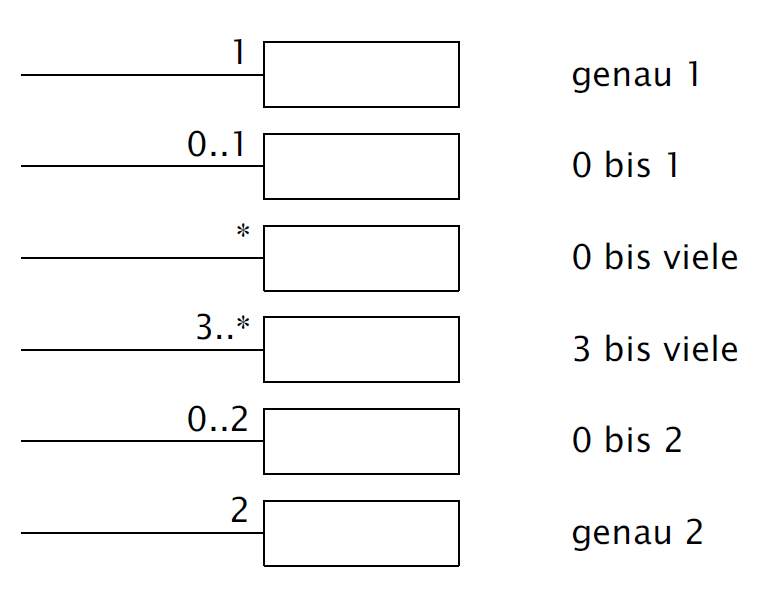
\includegraphics[width=6cm]{./bilder/Notation_Multiplizitaet.png}}
    \item[abgeleitete Assoziation] 
      Die Abhängigkeiten sind bereits durch andere Assoziationen beschrieben worden.
      Präfix "`\textbf{/}"'
    \item[Assoziationsname] 
      Beschreibt im Allgemeinen nur eine Richtung der Assoziation. 
    \item[Leserichtung] 
      Angabe beim Assoziationsnamen. Wird mit ausgefülltem schwarzem Dreieck ($\RHD$) dargestellt.
    \item[Sichtbarkeit] 
      Vor dem Rollenname geschriben. -private \#protected +public $\sim$package
    \item[Eigenschaftswert der Assoziation] 
      OOA: siehe \Balzert{45}\\
      OOD: siehe \Balzert{288}
      
    \parbox{5cm}{
      \item[Rolle]
        Information oder die Bedeutung/Funktion einer Klasse in Beziehung zu einer anderen.
      \item[Rollenname]
        Jeweils am Ende der Assoziationsrichtung von der Klasse, 
        deren Bedeutung sie beschreibt. Kann zur Verständlichkeit beitragen.}
    \hspace{0.5cm}
    \parbox{8cm}{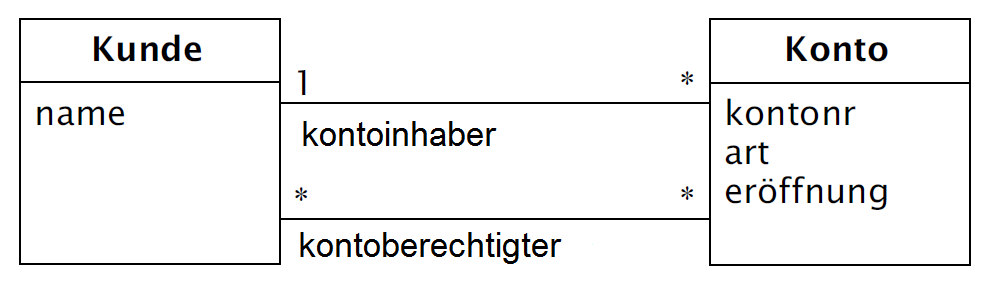
\includegraphics[width=8cm]{./bilder/Rolle.png}}
  \end{description}

\subsection{Generalisierung (Vererbung) \balzert{52}}
  Beschreibt die Beziehung zwischen einer allgemeinen Klasse (Basisklasse) und
  einer spezialisierten Klasse. Die spezialisierte Klasse ist vollständig
  konstistent mit der Basisklasse, enthält aber zusätzliche Informationen
  (Attribute, Operationen, Assoziationen). Jedes Objekt der Unterklasse \textbf{ist ein} 
  Objekt der Oberklasse.
  
  \begin{description}
    \item[Einfachvererbung]
    \item[Mehrfachvererbung]
    \item[Generalisierung] 
      Die spezialisierte Klasse erweitert die Liste der
      Attribute, Operationen und Assoziationen der Basisklasse
    \item[Generalisierungsmenge] 
      spezifiziert, nach welchen Kriterien eine Generalisierungstruktur erstellt wird.
      (z.B. nach Tätigkeit, Job, etc.)
  \end{description}

\subsection{Aktivität \balzert{69}}
  Eine Aktivität beschreibt die Auführung von Funktionalität bzw. Verhalten.

\subsection{Zustandsautomat \balzert{87}}
  Zustandsdiagramm (finit state diagram)
 

\newpage

\subsection{Use-Case Diagramm \balzert{62}}
	Ein Use-Case spezifiziert eine Sequenz von Aktionen
	\begin{description}[leftmargin=2cm]
		\item[Akteur]
      \parbox{6cm}{
        ist eine Rolle, die ein Benutzer des Systems spielt. Jeder Akteur hat einen 
        Einfluss uaf das System. Befindet sich stets ausserhalb des Systems}
      \hspace{0.5cm}
      \parbox{9cm}{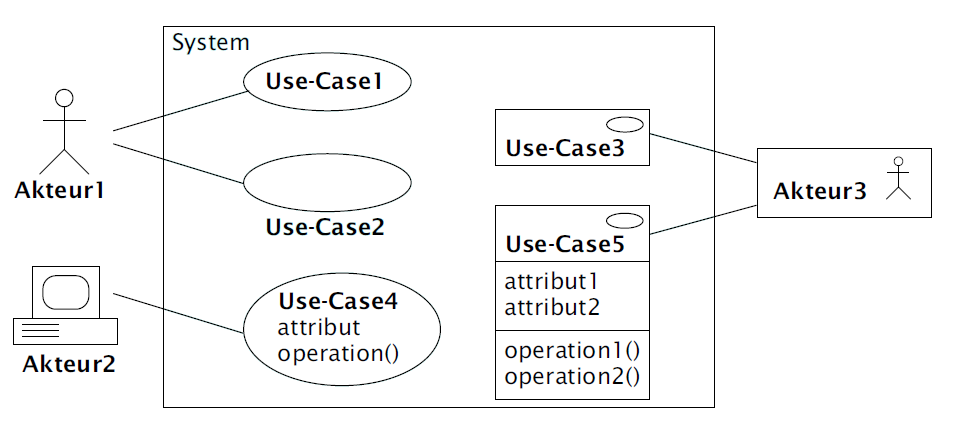
\includegraphics[width=9cm]{./bilder/UseCase_Notation.png}}
    \item[Schablone]
      \begin{itemize}[leftmargin=4cm]
        \item[\textit{Ziel:}]
          globlae Zielsetzung bei erfolgreicher Ausführung des Geschäftsprozesses.
        \item[\textit{Kategroie:}]
          primär, sekundär, optional
        \item[\textit{Vorbedingung:}]
          erwarteter Zustand, bevor der Use-Case beginnt.
        \item[\textit{Nachbedingung Erfolg:}]
          erwarteter Zustand, nach erfolgreicher Ausführung des Use-Cases (Ergebnis)
        \item[\textit{Nachbedingung Fehlschlag:}]
          erwarteter Zustand, wenn das Ziel nicht erreicht werden kann
        \item[\textit{Akteure:}]
          Rollen von Personen oder anderen Systeme, die den Use-Case auslösen
          oder daran beteiligt sind.
        \item[\textit{Auslösendes Ereignis:}]
          Wenn dieses Ereignis eintritt, dannn wird der Use-Case initiiert.
        \item[\textit{Beschreibung:}]
          \begin{enumerate}[leftmargin=0.5cm]
            \item Erste Aktion
            \item Zweite Aktion
          \end{enumerate}
        \item[\textit{Erweiterungen:}]
          \begin{enumerate}[leftmargin=0.5cm]
            \item[1a] Erweiterung des Funktionsumfangs der ersten Aktion
          \end{enumerate}
        \item[\textit{Alternativen:}]
          \begin{enumerate}[leftmargin=0.5cm]
            \item[1a] Alternative Ausführung der ersten Aktion
            \item[1b] Weitere Alternativen zur ersten Aktion
          \end{enumerate}
        \item[\Balzert{68}]
      \end{itemize}
	\end{description}


\subsection{Szenario \balzert{80}}
  Ein Szenario ist eine Sequenz von Verarbeitungsschritten, die unter bestimmten
  Bedingungen auszuführen ist.\\
  Die Szenarien lassen sich in zwei Kategorien unterteilen, die die eine erfolgreiche Bearbeitung
  des Use-Case beschreiben und jene Szenarien welche zu einem Fehlschlag führen. \\
  
  \textbf{Diagrammübersicht:}
  \begin{itemize}[leftmargin=0.5cm]
    \item Sequenzdiagramm $\rightarrow$ siehe \Balzert{81}
    \item Kommunikationsdiagramm $\rightarrow$ siehe \Balzert{85}
    \item Timing-Diagramm
    \item Interaktionsübersichtsdiagram
  \end{itemize}
  
\subsection{Analyseprozess \balzert{130}}
  Der Analyseprozess beschreibt die methodeische Vorgehensweise zur Erstellung eines
  obejektorientierten Analysemodells.\\
  
  Es besteht aus
  \begin{description}
    \item[Markoprozess]
      Der Makroprozess legt die methodischen Schritte fest, sprich in welcher
      Reihenfolge die Checklisten abgearbeitet werden $\rightarrow$ siehe \Balzert{132}
    \item[Checklisten]
      siehe \Balzert{133}
  \end{description}
  
  
\section{OOD}
\subsection{Ziel des Entwurfs}
  \begin{itemize}[leftmargin=0.5cm]
    \item Spezifizierte Anwendung auf einer Plattform unter den geforderten technischen
      Randbedingungen zu realisieren
    \item Entwurf liegt noch in einem höheren Abstraktionsniveau als in der Implementierung
    \item In der Entwurfsphase wird das OOD-Modell unter den Gesichtspunkten
      der Effizienz und Standardisierung konzipiert.
    \item Jede entworfene Klasse kann direkt implementiert werden
    \item Das OOD-Modell baut auf dem OOA-Modell auf
    \item Die Namen in dem OOD-Modell sollten der Syntax der jeweiligen Programmiersprache
      entsprechen.
  \end{itemize}

  \parbox{9cm}{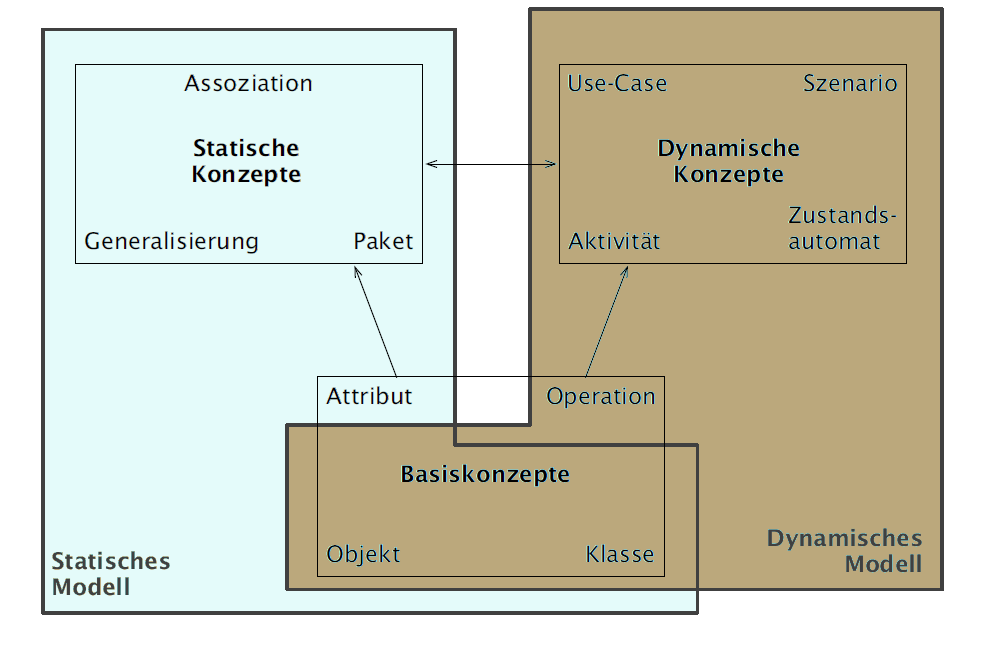
\includegraphics[width=9cm]{./bilder/Konzepte.png}}
  
\subsection{Klassen \balzert{252}}
  \begin{description}
    \item[parametrisierte Klasse]
      Template
    \item[Container Klasse]
      dient zur Verwaltung von einer Menge von Objekten einer anderen Klasse
      (typischerweise als Array implementiert)
    \item[Schnittstelle \Balzert{256}]
      \parbox{5cm}{ähnlich wie abstrakte Klasse, aber \textbf{keine Operation} ist implementiert}
      \hspace{0.5cm}
      \parbox{7cm}{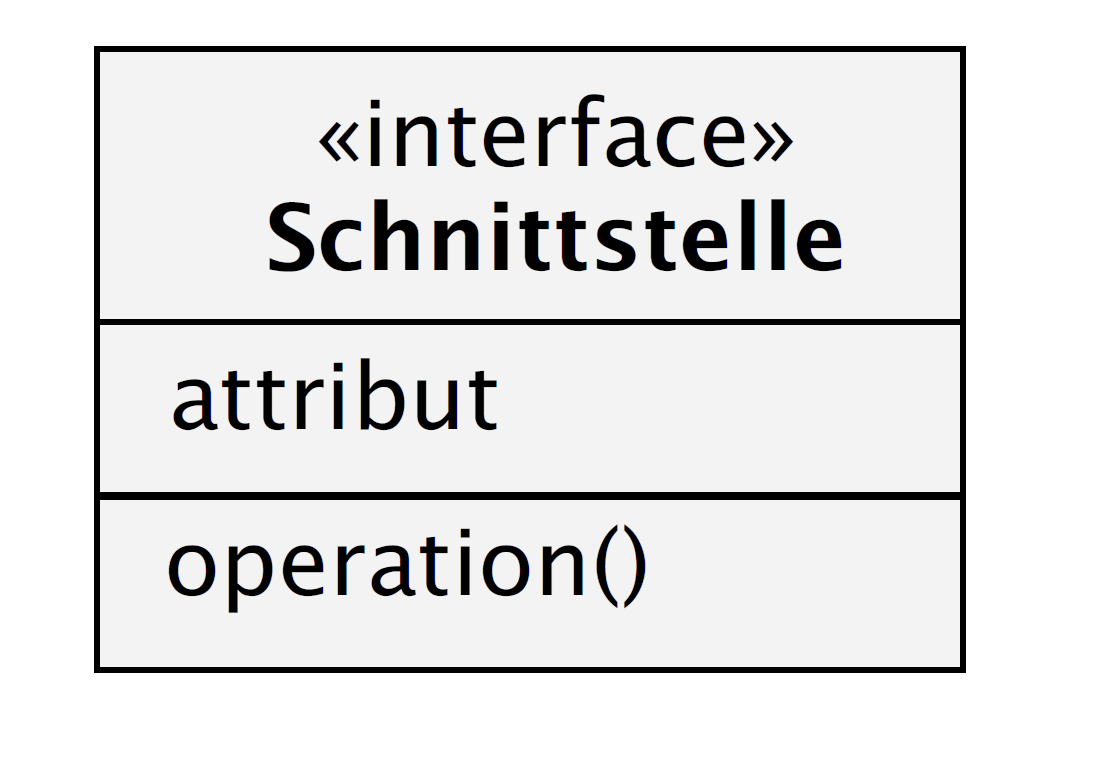
\includegraphics[width=7cm]{./bilder/Schnittstelle.png}}
    \item[Implementierung]
      siehe \Balzert{258, 259}
  \end{description}
  

\subsection{Attribut \balzert{261}}
  \begin{description}
    \item[Sichtbarkeit]
      \begin{itemize}[leftmargin=0.5cm]
        \item[$+$] public
        \item[$\#$] protected
        \item[$-$] privat
        \item[$\sim$] package
      \end{itemize}
    \item[Klassenattribute]
      werden durch \underline{Unterstrichen} gekennzeichnet und mit \textbf{static} implementiert
    \item[Notation]
      Sichtbarkeit / \textbf{name} : Typ [Multiplizität] = Anfangswert $\lbrace$Eigenschaftswert$\rbrace$ \\
    \parbox{6cm}{
      \item[Eigenschaftswerte]
        siehe \Balzert{263}
      \item[Implementation]
        siehe \Balzert{264} }
    \parbox{6cm}{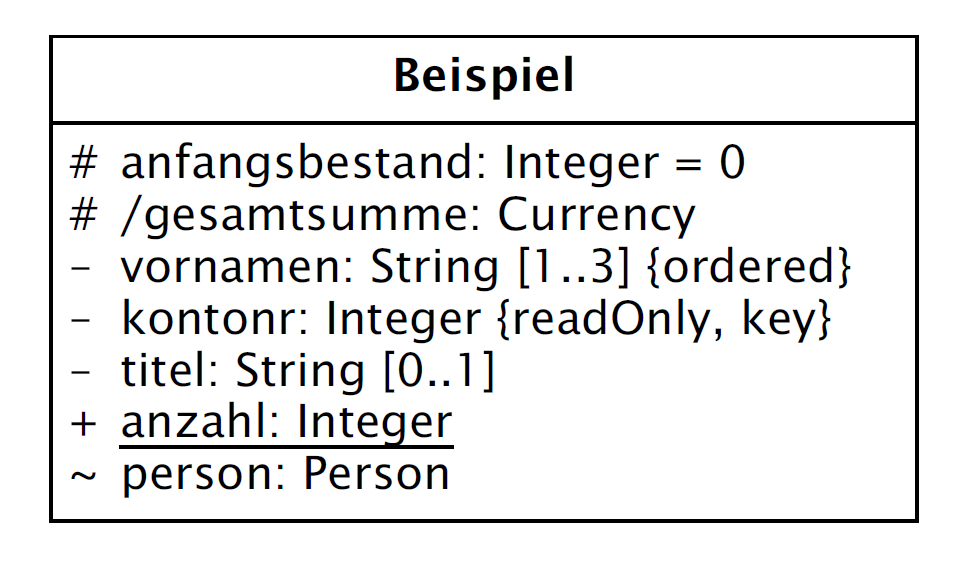
\includegraphics[width=5cm]{./bilder/Notation_Attribute.png}}
  \end{description}
  
  
\subsection{Operationen \balzert{266}}
  \begin{description}
    \item[Notation]
      Sichtbarkeit \textbf{name} (Parameterliste) : Ergenistyp $\lbrace$Eigenschaftswert$\rbrace$
    \item[Parameter]
      Richtung parametername : Typ [Multiplizität] = Anfangswert $\lbrace$Eigenschaftswert$\rbrace$ \\
      \parbox[t]{2cm}{Richtung: }
      \parbox[t]{2cm}{$\bullet$ in \\ $\bullet$ out \\ $\bullet$ inout \\ $\bullet$ return} \\[6pt]
      siehe \Balzert{267}
    \item[Eigenschaftswerte]
      siehe \Balzert{268}
    \item[Implementation]
      siehe \Balzert{269}
  \end{description}
  
\subsection{Komponente \balzert{273}}
  \begin{minipage}{12cm}
    Eine Komponente ist ein Softwarebaustein, der über klar definierte Schnittstellen, Verhalten bereitstellt.
    Das Innenleben der Komponente bleibt gegen aussen verborgen
  \end{minipage}
  \begin{minipage}{6cm}
    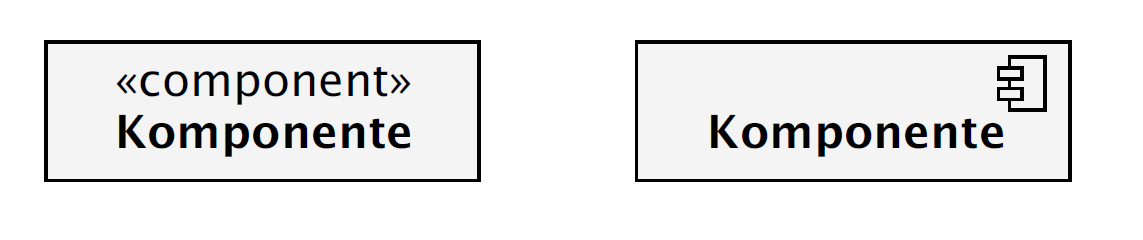
\includegraphics[width=6cm]{./bilder/Komponente.png}
  \end{minipage}
  

\subsection{Assoziation \balzert{284}}
  By-Value wird automatisch mit einer Komposition erstellt.
  \begin{description}[leftmargin=3.5cm]
    \item[Navigierbarkeit]
      \parbox{5cm}{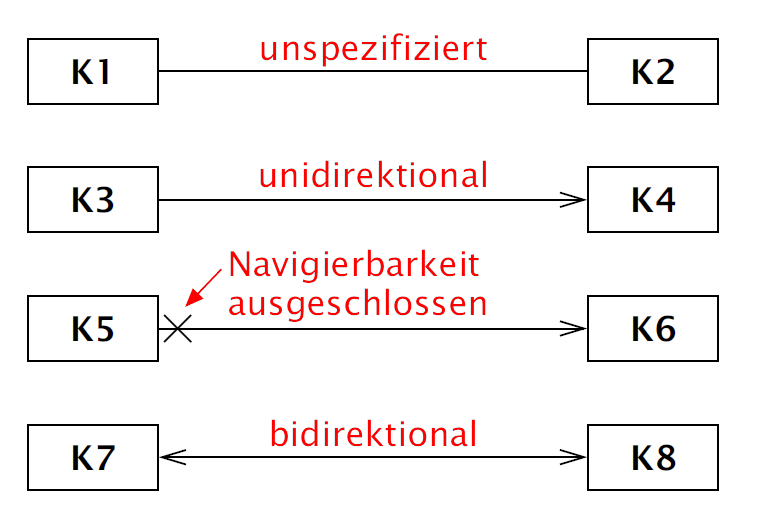
\includegraphics[width=5cm]{./bilder/Navigierbarkeit.png}}
      \hspace{3cm}
      \parbox{8cm}{
      \textbf{Auflösen einer Assoziationsklasse}\\
      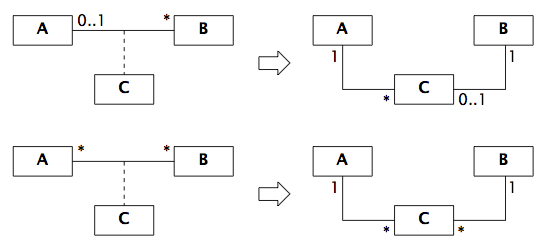
\includegraphics[width = 6cm]{./bilder/Aufloesen_Assoziationsklasse}}
      
    \item[Notation]
      \parbox{8cm}{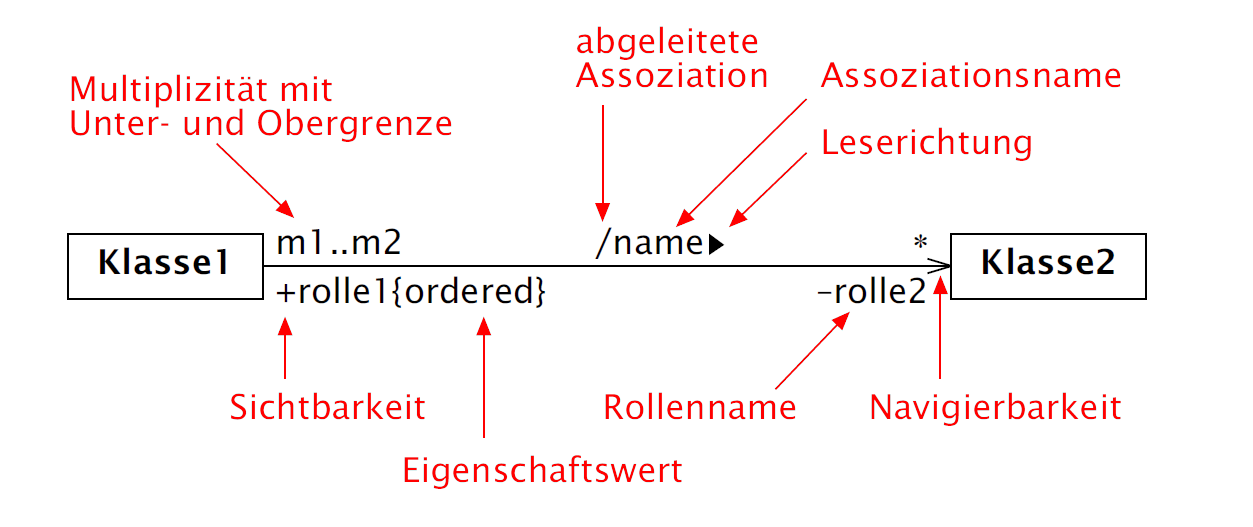
\includegraphics[width=8cm]{./bilder/Notation_Assozi_1.png}}
      \parbox{7cm}{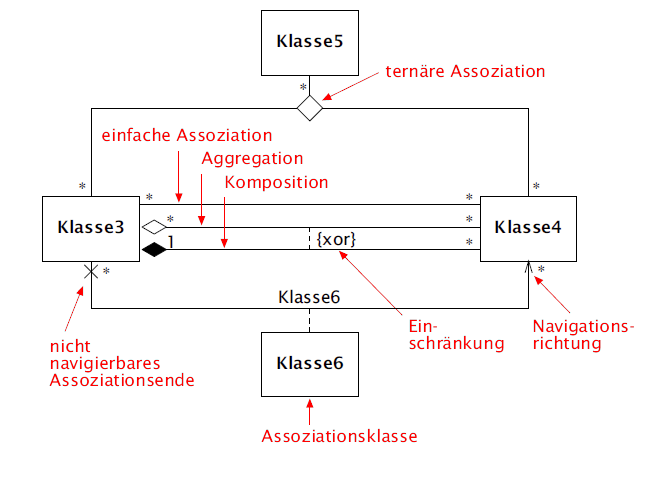
\includegraphics[width=7cm]{./bilder/Notation_Assozi_2.png}}
    \item[Eigenschaftswerte]
      siehe \Balzert{288}
    \item[Implementation]
      siehe \Balzert{291}
  \end{description}

\subsection{Polymorphismus \balzert{293}}
  Polymorphismus ermöglicht es, den gleichen Namen für gleichartige Operationen,
  in verschiedenen Klassen zu gebrauchen.
  \begin{description}
    \item[]
    \item[Notation]
      Operation \textit{kursiv} schreiben
    \item[Deklaration]
      mit \textbf{virtual} deklarieren
    \item[Implementation]
      siehe \Balzert{298}
  \end{description}
  
\subsection{Generalisierung \balzert{300}}
  \begin{description}
    \item[Generalisierungseigenschaften]
      siehe \Balzert{302}
    \item[Notation]
      \parbox{15cm}{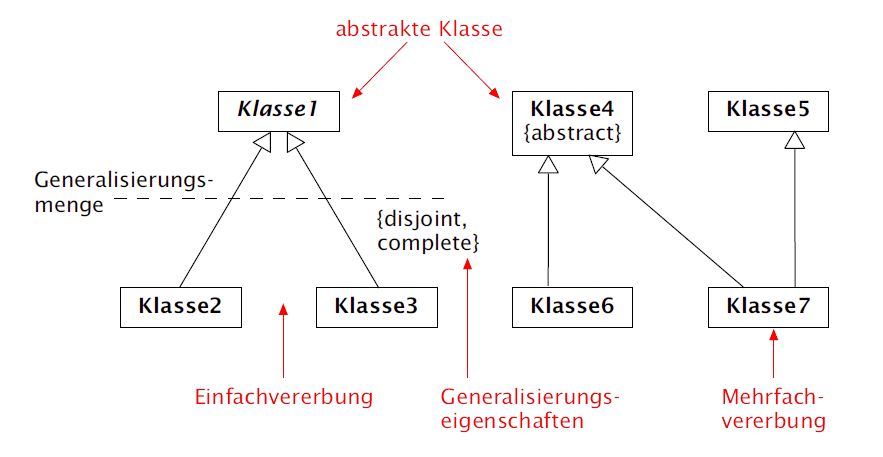
\includegraphics[width=8cm]{./bilder/Notation_Generalisierung.png}}
    \item[Implementation]
      siehe \Balzert{305}
  \end{description}
  

\subsection{Szenario \balzert{327}}
  bezieht sich auf Sequenzdiagramme
  \begin{description}
    \item[synchrone Nachricht]
      Der Sender wartet bis der Empfänger die Verarbeitung komplett durchgeführt hat.
    \item[asynchrone Nachricht]
      Der Sender wartet \textbf{nicht} bis auf den Empfänger, sondern setzt seine Verarbeitung
      parallel fort.
    \item[kominierte Fragmente]
      siehe \Balzert{331}
    \item[Notation]
      \parbox{15cm}{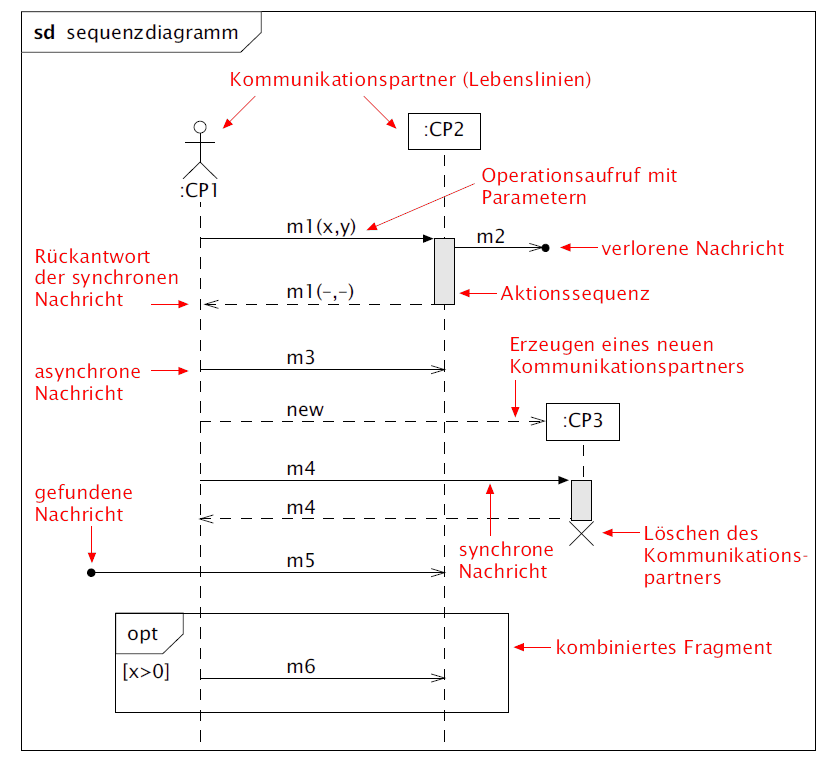
\includegraphics[width=10cm]{./bilder/Notation_Sequanzdia.png}}
  \end{description}
  
\subsection{Entwurfsmuster \balzert{355}}

\end{document}
